% \documentclass[pdftex,10pt,a4paper,oneside]{book}
%Can change the pt, papersize etc.
\documentclass[oneside]{book}
\usepackage{blindtext}
\usepackage[T1]{fontenc}
\usepackage[utf8]{inputenc}
% \usepackage{algorithm}
% \usepackage{algorithmic} %Algorithm styles, need to be nested for the example shown
\usepackage{fancyhdr} %For our headers
\usepackage{graphicx} %Inserting images
\usepackage{lipsum}  %Blank text fill, delete me when finished
\usepackage{setspace} %Spacing on the front page for crest and titles
\usepackage[]{fncychap} % Styles can be Sonny, Lenny, Glenn, Conny, Rejne, Bjarne and Bjornstrup
\usepackage[hyphens]{url} %Deals with hyphens in urls to make them clickable
\usepackage{xcolor} %Great if you want coloured text
\usepackage{tabularx}
\usepackage{appendix} %Take a wild guess slick

%KEEP THIS ONE LAST it's quite buggy, it allows you to click on links within the pdf and web links without changing the colour. The mouse cursor simply changes its icon to indicate to the user. Great tool - still awkward
\usepackage[hidelinks]{hyperref}


%This will tell the compiler to do the header style, page and spacing between the header and text
\fancyhf{}
\renewcommand{\headrulewidth}{0.2pt}
\newcolumntype{P}[1]{>{\centering\arraybackslash}p{#1}}

\usepackage{float} 
\usepackage{import}
\graphicspath{ {figures/} }
\usepackage{array}
\usepackage{xcolor,colortbl}
\definecolor{Gray}{gray}{0.85}


\usepackage{tabularx}
    \newcolumntype{L}{>{\raggedright\arraybackslash}X}

\usepackage[utf8]{inputenc}
\usepackage{fourier} 
\usepackage{array}
\usepackage{makecell}
\usepackage{array,multirow}

\renewcommand\theadalign{bc}
\renewcommand\theadfont{\bfseries}
\renewcommand\theadgape{\Gape[4pt]}
\renewcommand\cellgape{\Gape[4pt]}
 

\newtheorem{defn}{Definition}[section]
\title{PCIe}
\author{Prepared by Design Team }
\date{January 2021}
% Specification
% for \\ PCIe Physical Layer\\

\begin{document}


\begin{titlepage}
    \begin{center}

\includegraphics[height=0.9in,width=3in]{images/mentor.png}
        \vspace*{3cm}
            
        \Huge
        Hardware Specification
        \\
            for
        \\
        PCIe Physical Layer Gen5
        \\
        \vspace{0.5cm}

        \vspace{1.5cm}
            
        \textbf{Prepared by Design Team}
            
         \vspace{8cm}
      
        % \huge
        % Department of Computer Systems Engineering\\
        % Faculty of Engineering at Ain Shams University\\
         January 2021
            
    \end{center}
\end{titlepage}

\pagenumbering{arabic}

\tableofcontents
\listoffigures
\listoftables
\chapter*{Revision history} 
\begin{tabularx}{1.2\textwidth} { 
  | >{\raggedright\arraybackslash}X 
  | >{\centering\arraybackslash}X 
  | >{\raggedleft\arraybackslash}X | }
 \hline
 \textbf{Revision Number} & \textbf{Date}& \textbf{Description} \\
 \hline
0.1 & 13/1/2021  & Initial Draft  \\ \hline
1.0 & 25/1/2021  & First resealed of specification \\ \hline
1.5 & 8/2/2021  & Second resealed of specification \\

\hline
\end{tabularx}
\pagebreak

\chapter{Introduction}

\section{Overview}

PCIe (peripheral component interconnect express) is an interface standard for connecting
high-speed components. Every desktop PC motherboard has a number of PCIe slots you
can use to add GPUs (aka video cards aka graphics cards), RAID cards, Wi-Fi cards or SSD (solid-state drive) add-on cards. The types of PCIe slots available in the PC will depend on the motherboard that we bought. 
 \newline
PCIe slots come in different physical configurations: x1, x4, x8, x16, x32. The number after the x tells how many lanes (how data travels to and from the PCIe card) that PCIe
slot has. A PCIe x1 slot has one lane and can move data at one bit per cycle. A PCIe x2 slot
has two lanes and can move data at two bits per cycle (and so on).
\newline 
PCIe x1 card can be inserted into a PCIe x16 slot, but that card will receive less
bandwidth. Similarly, a PCIe x8 card can be inserted into a PCIe x4 slot, but it’ll only work
with half the bandwidth compared to if it was in a PCIe x8 slot.\newline
PCIe has undergone several large and smaller revisions, improving on performance and
other features. So there are several generations and in this spec we will design and
implement the physical layer of gen 5. The official PCIe 5.0 standard came out in May
2019. It will bring 128 GB/s of throughput. The specification is backwards compatible with
previous PCIe generations and also includes new features, including electrical changes to
improve signal integrity and backward-compatible CEM connectors for add-in cards.
Before designing and implementing the architecture of gen 5, there is an overview to
discuss the general basic concepts of PCIe.
\section{PCIe}
\noindent\rule{13cm}{0.4pt}
\begin{defn}
PCIe is an interface standard for connecting high-speed components. It is a serial bus
model. 
\end{defn}
\noindent\rule{13cm}{0.4pt}
There were many problems limiting the performance of the parallel bus:
\begin{itemize}
    \item  Flight time must be less than the clock period or the model won’t work.
\item  Clock skew
\item  Signal skew
\end{itemize}
But the serial transport got over these problems for example flight time becomes nonissue as the clock that will latch the data into the receiver is built into the data stream
and no external reference clock, so for the same reason no clock skew. Also, signal skew
is eliminated within a lane because there is only one bit of data being sent. 

\section{Lane}

\noindent\rule{13cm}{0.4pt}
\begin{defn}
A lane is composed of two differential signaling pairs, one pair for receiving data and the other for transmitting. Thus, each lane is composed of four wires.
\end{defn}
\noindent\rule{13cm}{0.4pt}
\newline
Number of lanes is called “link width” and is represented as x1, x2, x4, x8, x16 and x32.
The tradeoff regarding the number of lanes: more lanes increase the bandwidth of the link but it also increases the cost, space requirement and power consumption.

\begin{figure}[H]
  \centering
  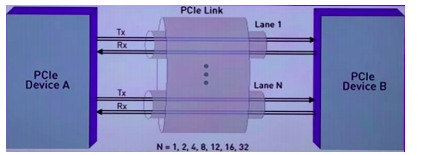
\includegraphics[width=100mm,height=60mm]{images/lane.png}
  \caption{PCIe Link}
  \label{lane}
\end{figure}

In the receiver, PLL circuit (phase locked loop) takes the incoming bit stream as a
reference clock and compares its timing or phase to that of an output clock that it has
created with a specified frequency. Based on the result of that comparison, the output
clock frequency is increased or decreased until a match is obtained, so the output clock
frequency precisely matches the clock that was used to transmit the data. \newline 

Each lane uses differential signaling, this improves noise immunity and reduced signal
voltage. Moreover, anything that will affect the signal will also affect the other by about
the same amount and in the same direction so the receiver won’t be affected by the
noise that affects the signals and will be able to distinguish the bits.

\section{Generations Speeds}

\begin{table}[H]
\caption{PCIe Generations Speeds for link width x16}
    \centering
    \begin{tabular}{|c|c|c|c|}
    \hline
    
    Version & Bandwidth & Gigatransfer & Frequency \\ \hline \hline
         PCIe 1.0  & 8 GB/s & 2.5 GT/s & 2.5 GHz \\ \hline
         PCIe 2.0  & 16 GB/s & 5 GT/s & 5 GHz \\ \hline
         PCIe 3.0  & 32 GB/s & 8 GT/s & 8 GHz \\ \hline
         PCIe 4.0  & 64 GB/s & 16 GT/s & 16 GHz \\ \hline
         PCIe 5.0  & 128 GB/s & 32 GT/s & 32 GHz \\ \hline
        %  PCIe 1.0  & 8 GB/s & 2.5 GT/s & 2.5 GHz \\ \hline
    \end{tabular}

    \label{tab:my_label}
\end{table}
Bandwidth calculations for link width x1:
\begin{equation}
    PCIe_{{B.W}_{Gen1}} = (2.5 Gb/s \times 2 \quad directions)/10 \quad bits \quad per \quad symbol = 0.5 \quad GB/s
\end{equation}
\begin{equation}
    PCIe_{{B.W}_{Gen2}} = (5 Gb/s \times 2 \quad directions)/10 \quad bits \quad per \quad symbol = 1 \quad GB/s
\end{equation}
\begin{equation}
    PCIe_{{B.W}_{Gen3}} = (8 Gb/s \times 2 \quad directions)/8 \quad bits \quad per \quad byte = 1 \quad GB/s
\end{equation}

\section{Topology}

A Topology is composed of point-to-point Links that interconnect a set of components.
This figure \ref{T} illustrates a single fabric instance referred to as a hierarchy – composed of a
Root Complex (RC), multiple Endpoints (I/O devices), a Switch, and a PCI Express to
PCI/PCI-X Bridge, all interconnected via PCI Express Links.

\begin{figure}[H]
  \centering
  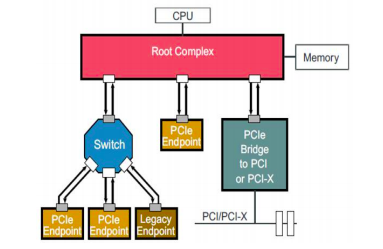
\includegraphics[width=100mm,height=80mm]{images/T.png}
  \caption{Topology}
  \label{T}
\end{figure}

\begin{itemize}
    \item  Root complex: it is the interface between the system CPU and the PCIe topology 
    \begin{itemize}
        \item  Root complex may support one or more PCI Express Ports. Each interface
defines a separate hierarchy domain. Each hierarchy domain may be
composed of a single Endpoint or a sub-hierarchy containing one or more
Switch components and Endpoints.
\item The capability to route peer-to-peer transactions between hierarchy
domains through a Root Complex is optional and implementation
dependent.
    \end{itemize}
    \item Switch: allows more devices to be attached to a single PCIe port, they act as a
packet routers and recognize which path a packet will need to take based on its
address or other routing information (may have several downstream ports but
only one upstream port).
\begin{figure}[H]
  \centering
  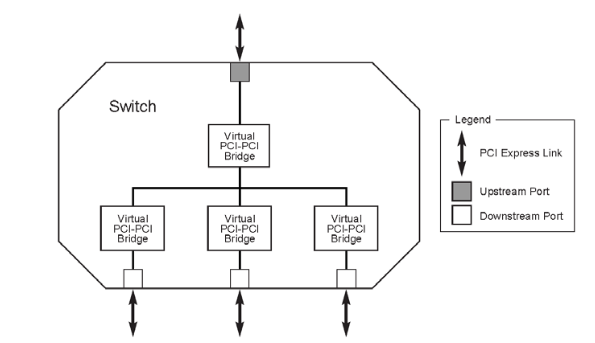
\includegraphics[width=100mm,height=80mm]{images/switch.png}
  \caption{switch}
  \label{lane}
\end{figure}
All Switches are governed by the following base rules:
\begin{itemize}
    \item Switches appear to configuration software as two or more logical PCI-to-PCI Bridges.
    \item Switch must forward all types of Transaction Layer Packets between any
set of Ports.
\item  Switch is not allowed to split a packet into smaller packets.
\end{itemize}
\item Bridge: provides interface to other buses such as PCI or PCI-X or even another
PCIe bus. \newline
Forward bridge $\longrightarrow$ allows older card to be plugged into a new system. \newline
Reverse bridge $\longrightarrow$ allows a new PCIe card to be plugged into an old PCI system.
\item End points: devices that act as initiators and completers of transactions on the
bus (they only implement a single upstream port). Endpoints are classified as
either legacy, PCI Express, or Root Complex Integrated Endpoints.
\end{itemize}
Root complex will appear to configuration software as PCI bus number zero and the PCIe
ports will appear as PCI to PCI bridges. In a similar way, a switch will appear to software
simply as a collection of bridges sharing a common bus. \newline
The advantage of this approach is that it allows the transaction routing to take place in
the same way it did for PCI.
\begin{figure}[H]
  \centering
  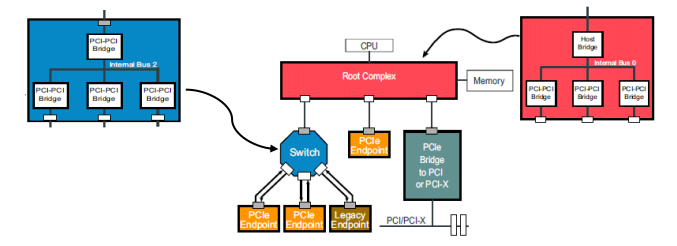
\includegraphics[width=150mm,height=80mm]{images/r.png}
  \caption{configuration software for PCIe}
  \label{fig:r}
\end{figure}

\section{Device layers}
The architecture of PCIe device is divided into three discrete logical layers: Transaction
Layer, Data Link Layer and Physical Layer. Each of these layers is divided into two
sections: one that processes outbound (to be transmitted) information and one that
processes inbound (received) information.
\begin{itemize}
    \item Transaction layer: creation of transaction layer packet (TLP) on the transmit side
and decoding on the receiver side. Also responsible for other 3 functions which
are flow control, quality of service and transaction ordering functionality.
    \item Data link layer: creation of data link layer packet (DLLP) on the transmit side and
decoding on the receiver side. Also, responsible for link error detection and
correction.
    \item Physical layer: creation of ordered set packet on transmit side and decoding on
the receiver side. It processes all 3 types of packets to be transmitted on the link
and processes packets received from the link also. Then packets are encoded and
serialized.
    \item Then link training and status state machine (LTSSM) of the physical layer is
responsible for link initialization and training.

\begin{figure}[H]
  \centering
  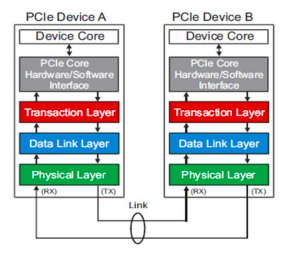
\includegraphics{images/D2.png}
  \caption{Device A and B connect by Link}
  \label{lane}
\end{figure}
    \item Note: switch port needs to implement all the layers as it
evaluates the contents of packets, to determine their
routing requires looking into the internal details of a packet
and that takes place in the transaction layer.

\begin{figure}[H]
  \centering
  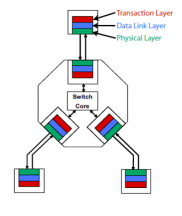
\includegraphics{images/Tl.png}
  \caption{Switch port}
  \label{lane}
\end{figure}
\end{itemize}

\section{layers interaction}
\begin{itemize}
    \item The contents of an outgoing request or completion packet from the device are
assembled in the transaction layer based on information presented by device core
logic. That information would usually include the type of command desired, the
address of the target device and amount of data to transfer.
\item The newly created packet is then stored in a buffer called a virtual channel until it
is ready for passing to the next layer. When the packet is passed down to data link
layer, additional information is added to the packet for error checking at the neighboring receiver and a copy is stored locally so we can send it again if a
transmission error occurs.
\item When the packet arrives at the physical layer, it is encoded and transmitted
differentially using all available lanes of the link.
\item When the packet arrives at the receiver, it decodes the incoming bits in the
physical layer and check for errors that can be seen at this level.
\item if there are no errors, then it forwards the resulting packet up to the data link
layer.
\item Again the resulting packet is checked, if no errors, then it will be forwarded up to
the transaction layer.
\item The packet is buffered, checked for errors and disassembled into the original
information so the contents can be delivered to the device core of the receiver.
\end{itemize}

\section{TLP packet}
\begin{figure}[H]
  \centering
  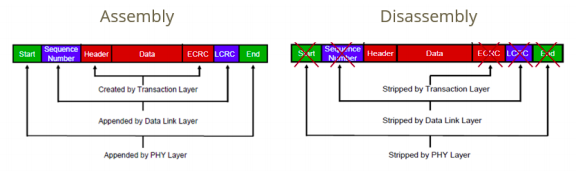
\includegraphics[width=160mm,height=40mm]{images/TLP.png}
  \caption{TLP}
  \label{lane}
\end{figure}
\section{DLLP packet}
They are transferred between data link layers of 2 neighboring devices on a link and the
transaction layer isn’t aware of these packets. Its size is 8 bytes (very small compared to
TLPs).
\begin{figure}[H]
  \centering
  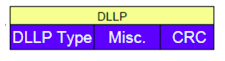
\includegraphics{images/DLLP.png}
  \caption{DLLP}
  \label{lane}
\end{figure}
Note: this DLLP differs from the structure of TLP at the data link layer 

\begin{figure}[H]
  \centering
  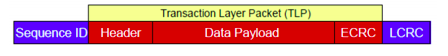
\includegraphics{images/TLP_link_layer.png}
  \caption{TLP at data link layer}
  \label{lane}
\end{figure}

\section{Physical layer}
It is divided into 2 portions:
\begin{enumerate}
    \item Logical $\longrightarrow$  contains the digital logic associated with preparing the packets for
serial transmission on the link and reversing the process for inbound packets.
\item Electrical  $\longrightarrow$ the analog interface that connects to the link and consists of
differential drivers and receivers for each lane.
\end{enumerate}

\begin{figure}[H]
  \centering
  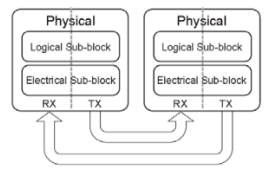
\includegraphics{images/phy.png}
  \caption{Physical Layer}
  \label{lane}
\end{figure}

\section{Logical sub-block}
It has two main sections: Transmit section that prepares outgoing information passed
from the Data Link Layer for transmission by the electrical sub-block, and Receiver
section that identifies and prepares received information before passing it to the Data
Link Layer. The logical sub-block and electrical sub-block coordinate the state of each
Transceiver through a status and control register interface or functional equivalent. The
logical sub-block directs control and management functions of the Physical Layer. PCI
Express uses 8b/10b encoding when the data rate is 2.5 GT/s or 5.0 GT/s. For data rates
greater than or equal to 8.0 GT/s, it uses a per-lane code along with physical layer
encapsulation.\newline \newline 
Logical sub-block contains mainly two logical blocks: MAC layer and PHY.

\section{PIPE Architecture}
\begin{itemize}
    \item Physical Interface for PCI Express Specification (PIPE) developed by Intel, has the
stated intent of providing a standard interface between the internal logic of a
PCIe design and the analog and high-speed circuitry required to implement the
serial link. The purpose of this functional separation is to allow ASIC and
integrated circuit designers to focus on the PCI Express device core, Transaction,
Data Link and logical Physical Layers, while relying on the PIPE-compliant physical
design (PHY) for the electrical interface of the design. 
    \item The PIPE spec defines standard functionality that a PIPE-compliant PHY needs to
implement, as well as a standard parallel interface between the PHY and the
internal logic referred to in the spec as MAC. 

    
\end{itemize}
\begin{figure}[H]
  \centering
  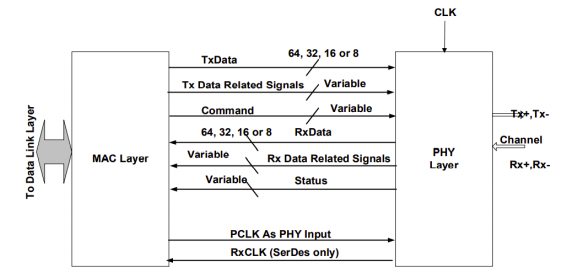
\includegraphics[width=100mm,height=80mm]{images/phymac.png}
  \caption{PHY/MAC Interface}
  \label{lane}
\end{figure}
\subsection{MAC Architecture}

The MAC contains many of the PCIe logical Physical Layer circuits (such as the Link
Training and Status State Machine (LTSSM), data scrambling, byte striping and
functions as the bridge between the DLL and the PHY/MAC interface)
\subsection{PHY/MAC Interface}
It is a parallel interface for transferring data to be transmitted on the PCIe bus.
The width of this parallel interface for bytes of data is shown as either be 8, 16, 32
or 64 bits in each direction.
\subsection{PHY Architecture}
\begin{itemize}
    \item It contains the 8b/10b encoder and decoder, elastic buffer, serializer and deserializer
    \item It contains the logic that controls the receiver detection and reports the detect
status to the MAC via the PHY/MAC Interface.
    \item It contains a Phase Lock Loop (PLL) to generate the internal, high speed clocks
used for the PHY based on the CLK input.
\end{itemize}
\subsection{PIPE PLL}
It generates the PCLK used in synchronizing the parallel PHY/MAC Interface based on the
CLK input.

\begin{figure}[H]
  \centering
  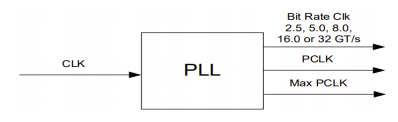
\includegraphics{images/pll.png}
  \caption{PLL}
  \label{lane}
\end{figure}

\subsection{LPIF Architecture}
The LPIF specifications defines common interface between the Link Layer and the logical
physical layer to facilitate interoperability, design and validation re-use between Link
Layers and Physical layers.
\begin{figure}[H]
  \centering
  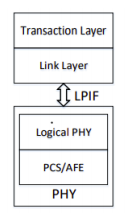
\includegraphics{images/lpif.png}
  \caption{LPIF}
  \label{lane}
\end{figure}

% \begin{figure}[H]
%   \centering
%   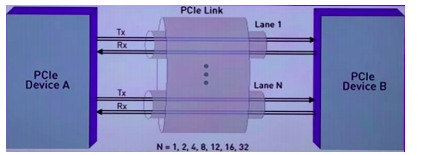
\includegraphics[width=100mm,height=80mm]{images/lane.png}
%   \caption{PCIe Link}
%   \label{lane}
% \end{figure}
\chapter{Features}
In this chapter, we will discuss the blocks and the states that we are going to support, design and implement.
% \section{Limitations}
% \begin{table}[H]
%     \caption{unsupported Blocks}
%     \centering
%   \begin{tabular}{ |m{26mm}|}
% \hline
% \rowcolor{Gray}
%  \multicolumn{1}{|c|}{\textbf{Unsupported Blocks}} 
% \\
% \hline


% 8/10b encoder \\ \hline 

% 128/130b encoder \\ \hline
% Serializer/ De-serializer \\ \hline
% Differential driver and receiver \\ \hline
% Elastic buffer logic \\ \hline 
% PLL (phase locked loop)
%  \\ \hline

% Lane de-skew delay circuit \\ \hline
% Block alignment and detect logic
%  \\ \hline
% Clock compensation \\ \hline
% \end{tabular}
% \end{table}
% \begin{table}[H]
%     \caption{unsupported states}
%     \centering
%   \begin{tabular}{ |m{26mm}|}
% \hline
% \rowcolor{Gray}
%  \multicolumn{1}{|c|}{\textbf{Unsupported States}} 
% \\
% \hline

% L1 \\ \hline 
%  L2 \\ \hline
% Hot Reset \\ \hline
% compliance  \\ \hline
% Loopback \\ \hline 
% Disable \\ \hline
% \end{tabular}

% \end{table}
\section{Supported Features}
\begin{table}[H]
    \caption{supported states}
    \centering
  \begin{tabular}{ |m{26mm}|}
\hline
\rowcolor{Gray}
\multicolumn{1}{|c|}{\textbf{
Supported States
} } \\
\hline

Detect \\ \hline 
Polling \\ \hline
Configuration\\ \hline
Recovery\\ \hline
L0\\ \hline 
L0s \\ \hline
\end{tabular}

\end{table}



\begin{table}[H]
    \caption{supported Blocks}
    \centering
  \begin{tabular}{ |m{26mm}|}
\hline
\rowcolor{Gray}
\multicolumn{1}{|c|}{\textbf{
Supported Blocks
} } 
\\
\hline


LPIF error handler \\ \hline 

LPIF control  \\ \hline
TxBuffer  \\ \hline
Ordered sets  \\ \hline
LTSSM  \\ \hline 
Byte Stripping / Unstripping 
 \\ \hline

Scrambler / De-scrambler  \\ \hline
PIPE register  
 \\ \hline
Arbiter/Mux \\ \hline
\end{tabular}
\end{table}


The LTSSM is composed of the following 11 states: Detect, Polling, Configuration, Recovery, L0, L0s, L1, L2, Hot Reset, Loopback, Disable. So here is a quick overview about the supported states:
\begin{enumerate}
    \item Detect \newline 
    It is the initial state of the physical layer, only used at Gen1 2.5 GT/s rate, or converted from the data link layer, or after reset, or from other states (Disable, Polling, Configuration, Recovery, etc.) Conversion. In short, the Detect state is the beginning of PCIe link training. In addition, Detect, as the name suggests, needs to implement detection work. Because in this state, the transmitting end TX needs to detect whether the receiving end RX exists and can work normally, if the detection is normal, it can enter other states. The Detect state mainly includes two sub-states: Detect.Quiet and Detect.Active.
    \item  Polling \newline 
    The purpose of this state is to "pair the cipher" and achieve barrier-free communication. After entering this state, the TS1 and TS2 OS sequences are sent between TX and RX to determine Bit Lock, Symbol Lock and solve the problem of Lane polarity reversal. The Polling state mainly includes three sub-states: Polling.Active, Polling.Configuration, Polling.Compliance.
    \item Configuration \newline 
    The content of this state is very simple. It is to determine the Link/Lane number by sending TS1 and TS2. Configuration contains 6 sub-states: Configuration.LinkWidth.Start, Configuration.LinkWidth.Accpet, Configuration.Lanenum.Wait, Configuration. Lanenum.Accpet, Configuration.Complete, Configuration.Idle

    \item Recovery \newline 
    When the PCIe link needs to be retrained, it enters the Recovery state. There are mainly the following situations:
\begin{itemize}
    \item When the PCIe link signal finds an error, the Bit Lock and Symbol Lock need to be adjusted

    \item  Exit from L0s state
    \item Speed Change. Because the first time you enter the L0 state, the rate is 2.5GT/s. When you need to adjust the rate to 5.0GT/s or 8.0GT/s, you need to enter the Recovery state for Speed Change. At this stage, Bit Lock, Symbol Lock, etc. Need to reacquire
    \item Need to readjust the Width of PCIe link
    \item Need to readjust the Width of PCIe link
    \item Only in Gen3 and Gen4, Equalization needs to be performed again.
\end{itemize}
    \item L0 \newline 
    This is the normal state (Normal and Full-Active State) of the link, and all TLP, DLLP and Ordered Sets can be sent and received normally. In this state, the rate can be 2.5GT/s or 5GT/s or higher (if the devices at both ends of the link support it and have undergone Re-Training).
    \item L0s \newline 
The ASPM (active-state power management) state is mainly used to reduce power consumption, and can enter this state when the bus is idle, and can quickly switch back to the L0 state from this state. When in the L0 state, when EIOS appears on the link, it means that it is about to enter the L0s state. When in the L0s state, when FTS appears on the link, the link will quickly complete bit lock and symbol lock, and enter the L0 state.
\end{enumerate}
\section{Supported Blocks}
\subsection{TxBuffer}
The ASPM (active-state power management) state is mainly used to reduce power consumption, and can enter this state when the bus is idle, and can quickly switch back to the L0 state from this state. When in the L0 state, when EIOS appears on the link, it means that it is about to enter the L0s state. When in the L0s state, when FTS appears on the link, the link will quickly complete bit lock and symbol lock, and enter the L0 state.
\subsection{Byte Stripping}
Bytes are striped across multiple lanes $\longrightarrow$ distribution of each byte to different lanes in turn to avoid different lanes with different data lengths.
%   \begin{figure}[H]
%   \centering
%   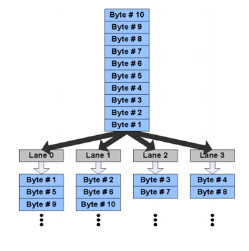
\includegraphics[width=80mm,height=80mm]{images/byte_str.png}
%   \caption{Byte Stripping}
  
%   \label{fig:pipe}
% \end{figure}
\subsection{Scrambler}
PCIe uses pseudo random data scrambling to spread off the RF energy in the frequency spectrum $\longrightarrow$ less electromagnetic interference (EMI). This is done by using a linear feedback shift registers on both the sender and receiver side. lfsr maintains an internal state machine which is the top flip-flops. An XOR operation is done between the state of the lfsr and the data $\longrightarrow$ resulting in a predictable and repeatable sequence of pseudo random data.
A parallel Scrambler performs 2 things: advance and apply. Advance means that the pattern changes, while apply means the XORing operation performed with this pattern.
\subsection{Ordered sets}
They are physical layer packets that only exists between Tx and Rx's physical layer.
\begin{itemize}
    \item TS1OS and TS2OS (Training Sequence 1 and 2)
    \item FTSOS (Fast Training Sequence)
    \item EIEOS (Electrical Idle Exit)
    \item EIOS (Electrical Idle)
    \item SOS (SKIP)
\end{itemize}
For more details about each block and how all the blocks interact together, see chapter \ref{4}.

% \begin{table}[H]
%     \caption{TX and Related signals}
%     \centering
%   \begin{tabular}{ |m{26mm}|m{10mm}|m{60mm}|  }
% \hline
% \rowcolor{Gray}
% \multicolumn{1}{|c|}{\textbf{Name} } 
% & \multicolumn{1}{|c|}{\textbf{Active Level}} 
% & \multicolumn{1}{|c|}{\textbf{Description}}\\
% \hline



% \end{tabular}
% \end{table}

\chapter{Signal Interface}
\clearpage
\section{PIPE Interface}

\label{sec:1}
\begin{table}[H]
    \caption{TX and Related signals}
    \label{tab:p1}
    \centering
  \begin{tabular}{ |m{26mm}|m{10mm}|m{60mm}|  }
\hline
\rowcolor{Gray}
\multicolumn{1}{|c|}{\textbf{Name} } 
& \multicolumn{1}{|c|}{\textbf{Active Level}} 
& \multicolumn{1}{|c|}{\textbf{Description}}\\
\hline
TxData[7:0] 
& 
N/A
&
Parallel data input bus. \\
\hline

TxDataValid
& 
N/A
&
This signal allows the MAC to instruct the PHY to ignore the data interface \newline
for one clock cycle. A value of one \newline
indicates the phy will use the data, a \newline
value of zero indicates the phy will not \newline
use the data. \\
\hline

TxElecIdle
& 
High
&
Forces Tx output to electrical idle when asserted
except in loopback.\newline \newline
Note: The MAC must always have TxDataValid
asserted when TxElecIdle transitions to either
asserted or deasserted; TxDataValid is a qualifier
for TxElecIdle sampling.
\\
\hline


TxDataK
& 
N/A
&
A value of zero indicates a
data byte, a value of 1 indicates a
control byte.\\
\hline


TxStartBlock
& 
N/A
&
This signals allow the MAC to tell
the PHY the starting byte for a 128b
block when value is 1. The starting byte for a 128b
block must always start with byte 0 of
the data interface. \\
\hline



TxSyncHeader[1:0]
& 
N/A
&

Provides the sync header for
the PHY to use in the next 130b block.
\newline \newline
$ 01 \longrightarrow $control byte \newline
$ 10 \longrightarrow $data byte

\\
\hline


TxDetectRx/ \newline Loopback
& 
High
&
Used to tell the PHY to begin a receiver detection
operation or to begin loopback \\
\hline



\end{tabular}

\end{table}


% Rx and related signal
\begin{table}[H]
    \caption{RX and Related signals}
    \label{tab:p2}
    \centering
  \begin{tabular}{ |m{26mm}|m{10mm}|m{60mm}|  }
\hline
\rowcolor{Gray}
\multicolumn{1}{|c|}{\textbf{Name} } 
& \multicolumn{1}{|c|}{\textbf{Active Level}} 
& \multicolumn{1}{|c|}{\textbf{Description}}\\
\hline
RxData[7:0] 
& 
N/A
&
Parallel data output bus. \\
\hline

RxDataValid
& 
N/A
&
This signal allows the PHY to instruct the MAC to ignore the data interface \newline
for one clock cycle. A value of one \newline
indicates the mac will use the data, a \newline
value of zero indicates the mac will not \newline
use the data. \\
\hline

RxElecIdle
& 
High
&
Indicates receiver detection of an
electrical idle. While deasserted
with the PHY in P2 (PCI Express
mode).
\\
\hline


RxDataK
& 
N/A
&
A value of zero indicates a
data byte, a value of 1 indicates a
control byte.\\
\hline


RxStartBlock
& 
N/A
&
This signals allow the PHY to tell
the MAC the starting byte for a 128b
block when value is 1. The starting byte for a 128b
block must always start with byte 0 of
the data interface. \\
\hline



RxSyncHeader[1:0]
& 
N/A
&

Provides the sync header for
the MAC to use in the next 130b block.
\newline \newline
$ 01 \longrightarrow $control byte \newline
$ 10 \longrightarrow $data byte

\\
\hline


RxValid
& 
High
&
Indicates symbol lock and valid
data on RxData and RxDataK and
further qualifies RxDataValid
when used.\\
\hline


RxStatus[2:0]
& 
N/A
&
Encodes receiver status and error
codes for the received data
stream when receiving data.\newline
\begin{tabular}{|m{2mm}|m{2mm}|m{2mm}|m{30mm}| }
 \hline
[0]&[1]&[2]& Description \\
     \hline
0 & 0 & 0 & Received data OK \\
     \hline
0 & 0 & 1 & 1 SKP added \\
     \hline
0 & 1 & 0 & 1 SKP removed \\
     \hline
0 & 1 & 1 & Receiver detected\\
     \hline
1 & 0 & 0 & Both $8B/10B$  $(128B/130B 6 )$ decode 
error and (optionally) 
Receive Disparity error \\
     \hline
1 & 0 & 1 & Elastic Buffer overflow \\
     \hline

1 & 1 & 0 & Elastic Buffer
underflow. \\
     \hline
1 & 1 & 1 & Receive disparity error
(Reserved if Receive
Disparity error is
reported with code
0b100)\\
     \hline

\end{tabular}

\\
\hline


\end{tabular}


\end{table}
\begin{table}[H]

    \centering
  \begin{tabular}{ |m{26mm}|P{18mm}|m{60mm}|  }
  \hline

RxStandby & Low & Controls whether the PHY RX is active when the
PHY is in P0 or P0s. \newline \newline
$0 \longrightarrow Active$ \newline
$1 \longrightarrow Standby$
\newline
 \\
     \hline
 RxStandbyStatus & Low &  The PHY uses this signal to indicate its
RxStandby state.
 \newline \newline
$0 \longrightarrow Active$ \newline
$1 \longrightarrow Standby$
\newline
\\
     \hline

\end{tabular}
\end{table}




\begin{table}[H]
    \caption{Clk and reset}
    \centering
  \begin{tabular}{ |m{26mm}|m{10mm}|m{60mm}|  }
\hline
\rowcolor{Gray}
\multicolumn{1}{|c|}{\textbf{Name} } 
& \multicolumn{1}{|c|}{\textbf{Active Level}} 
& \multicolumn{1}{|c|}{\textbf{Description}}\\
\hline
 Reset\# & Low & Resets the transmitter and receiver. This signal
is asynchronous. \\
\hline

 CLK & Edge & This differential Input is used to generate
the bit-rate clock for the PHY transmitter
and receiver.\\
\hline
 PCLK & Rising Edge & All data movement across the parallel
interface is synchronized to this clock.\\
\hline

\end{tabular}
\end{table}


\begin{table}[H]
    \caption{Commands and Status signals}
    \centering
  \begin{tabular}{ |m{26mm}|m{10mm}|m{60mm}|  }
\hline
\rowcolor{Gray}
\multicolumn{1}{|c|}{\textbf{Name} } 
& \multicolumn{1}{|c|}{\textbf{Active Level}} 
& \multicolumn{1}{|c|}{\textbf{Description}}\\
\hline
 
PowerDown[3:0] M2P  & N/A & Power up or down the transceiver. Power states
PCI Express Mode: \newline
\begin{tabular}{|m{2mm}|m{2mm}|m{2mm}|m{2mm}|m{30mm}|}
 \hline
[0]&[1]&[2]&[3]& Description \\
     \hline
     
0& 0 & 0 & 0 & P0, normal operation \\
     \hline
0& 0 & 0 & 1 & P0s, low recovery time
latency, power saving state \\
     \hline

0& 0 & 1 & 0 & P2, lowest power state\\
     \hline

\end{tabular}

\\
\hline

 
Rate[3:0] \newline M2P
 & N/A & 
 Control the link signaling rate.
 
 \begin{tabular}{|c|c|}
    \hline
     Value & Description  \\ \hline
     0  & Use 2.5 GT/s signaling rate \\ \hline
     1 & Use 5 GT/s signaling rate \\ \hline
     2 & Use 8 GT/s signaling rate\\ \hline
     3 & Use 16 GT/s signaling rate\\ \hline
     4 & Use 32 GT/s signaling rate\\ \hline
 \end{tabular}
\\
\hline
 PHY Mode[3:0] \newline M2P & N/A & PHYMode[1:0]
 \newline \newline
 $0 \longrightarrow PCI Express $
 \newline
 \\
\hline

\end{tabular}
\end{table}

\begin{table}[H]

    \centering
  \begin{tabular}{ |m{26mm}|P{18mm}|m{60mm}|  }
  
\hline
 PhyStatus \newline P2M & High & Used to communicate completion
of several PHY functions including
stable PCLK and/or Max PCLK
(depending on clocking mode)
after Reset\# deassertion, power
management state transitions,
rate change, and receiver
detection.\\
\hline

Width[1:0] & N/A &Controls the PIPE data path width. \newline 
\begin{tabular}{|c|c|}
\hline
    Value  & Datapath Width  \\ \hline
    0 &  8 bits \\ \hline
    1 & 16 bits \\ \hline
    2 & 32 bits \\ \hline
\end{tabular}
\\
\hline
PCLK Rate[4:0] & N/A & Control the PIPE PCLK rate. \newline
\begin{tabular}{|c|c|}
\hline
    Value  & clk rate  \\ \hline
    0 & 32.25 Mhz \\ \hline
    1 &  62.5 Mhz \\ \hline
    2 & 125 Mhz \\ \hline
    3 & 250 Mhz \\ \hline
    4 & 500 Mhz \\ \hline
    5 & 1000 Mhz \\ \hline
    6 & 2000 Mhz \\ \hline
    7 & 4000 Mhz \\ \hline
    
    
\end{tabular}
\\
\hline

PclkChangeAck \newline M2P & High & 
Only used when PCLK is a PHY input.
Asserted by the MAC when a PCLK rate
change or rate change or, if required,
width change is complete and stable. \newline 

After the MAC asserts PclkChangeAck
the PHY responds by asserting
PhyStatus for one cyle and de-asserts
PclkChangeOk at the same time as
PhyStatus. The controller shall deassert
PclkChangeAck when PclkChangeOk is
sampled low.

\\
\hline
PclkChangeOk \newline P2M & High &
Only used when PCLK is a PHY
input. Asserted by the PHY when
it is ready for the MAC to change
the PCLK rate or Rate.
\\
\hline
\end{tabular}
\end{table}



\begin{table}[H]
    \caption{Message Bus Interface Signals}
    \centering
  \begin{tabular}{ |m{30mm}|m{10mm}|m{60mm}|  }
\hline
\rowcolor{Gray}
\multicolumn{1}{|c|}{\textbf{Name} } 
& \multicolumn{1}{|c|}{\textbf{Direction}} 
& \multicolumn{1}{|c|}{\textbf{Description}}\\
\hline

M2P\_MessageBus[7:0] & Input & The MAC multiplexes command, any
required address, and any required data
for sending read and write requests to
access PHY PIPE registers and for
sending read completion responses and
write ack responses to PHY initiated
requests.  \\ \hline 
P2M\_MessageBus[7:0] & Output & The PHY multiplexes command, any
required address, and any required data
for sending read and write requests to
access MAC PIPE registers and for
sending read completion responses and
write ack responses to MAC initiated
requests.  \\ \hline 

\end{tabular}
\end{table}



\section{LPIF Inteface}
\label{sec:2}
\begin{table}[H]
\label{tab:l1}
    \caption{LPIF Interface Signals}
    \centering
  \begin{tabular}{ |P{26mm}|P{10mm} | m{60mm}|  }
\hline
\rowcolor{Gray}
\multicolumn{1}{|c|}{\textbf{Name} } 

& \multicolumn{1}{|c|}{\textbf{Active Level}}
& \multicolumn{1}{|c|}{\textbf{Description}}
\\
\hline
lclk & High &Link Clock: The clock frequency the LPIF interface operates at.
The Link Clock is an input to signal to both the Link Layer as well as the Logical PHY.\\ \hline

pl\_trdy & High & LIndicates Physical Layer is ready to accept data. Data is accepted when pl\_trdy, lp\_valid, and lp\_irdy are asserted together.\\ \hline


lp\_irdy & High & Link Layer to Physical Layer indicating Link Layer is ready to transfer data. lp\_irdy must not be presented by the upper layers when pl\_state\_sts is RESET.\\ \hline


lp\_valid [LP\_NVLD-1:0] & High & Link Layer to Physical Layer indicates data valid on the corresponding lp\_data bytes.
‘LP\_NVLD’ equals the number of valid bits. The bytes of lp\_data associated with a
specific bit of lp\_valid is implementation specific. When lp\_irdy is asserted, at least one
of the bits of lp\_valid must be asserted.\\ \hline
pl\_data [NBYTES-1:0][7:0] & N/A &
Physical Layer to Link Layer Data, where ‘NBYTES’ equals number of bytes determined
by the supported data bus for the LPIF interface. \\ \hline
pl\_valid [PL\_NVLD-1:0] & High &
Physical Layer to Link Layer indicates data valid on pl\_data. ‘PL\_NVLD’ equals the
number of valid bits. The bytes of pl\_data associated with a specific bit of pl\_valid is
implementation specific.\\ \hline
pl\_stallreq & High & Physical Layer request to Link Layer to flush all packets for state transition \\ \hline
lp\_data [NBYTES-1:0][7:0] & N/A & Link Layer to Physical Layer Data, where ‘NBYTES’ equals number of bytes determined
by the data width for the LPIF instance.
\\ \hline

\end{tabular}
\end{table}

\begin{table}[H]

    \centering
  \begin{tabular}{ |m{26mm}|P{18mm}|m{60mm}|  }
  \hline

\hline
lp\_stallack & High & Link Layer to Physical layer indicates that the packets are aligned (if pl\_stallreq was
asserted) and logPHY may begin state transitions. \\ \hline 
lp\_state\_req[3:0] & N/A & 
Link Layer Request to Logical Physical Layer to request state change.
Encodings as follows: \newline
0000: NOP \newline 
0001: Active \newline 
0010: Active.L0s \newline 
0011: Deepest Allowable PM State [L1 Substates only] \newline 
0100: L1.1 \newline 
0101: L1.2 \newline 
0110: L1.3 \newline 
0111: L1.4 \newline 
1000: L2 \newline 
1001: LinkReset \newline 
1010: Reserved \newline 
1011: Retrain \newline 
1100: Disable \newline 
\\ \hline
pl\_state\_sts[3:0] & N/A &
Physical Layer to Link Layer Status indication of the Interface.
Encodings as follows:
\newline
0000: NOP \newline 
0001: Active \newline 
0010: Active.L0s \newline 
0011: Deepest Allowable PM State [L1 Substates only] \newline 
0100: L1.1 \newline 
0101: L1.2 \newline 
0110: L1.3 \newline 
0111: L1.4 \newline 
1000: L2 \newline 
1001: LinkReset \newline 
1010: Reserved \newline 
1011: Retrain \newline 
1100: Disable \newline
\\ \hline
pl\_lnk\_cfg[2:0] & N/A &
Width of the Port: This bit field indicates the width of the port as determined by the Link
initialization: \newline
000 – x1 \newline
001 – x2 \newline
010 – x4 \newline
011 – x8 \newline
100 – x12 \newline 
101 – x16 \newline
110 – x32 \newline

\\ \hline
\end{tabular}
\end{table}


\begin{table}[H]

    \centering
  \begin{tabular}{ |m{26mm}|P{18mm}|m{60mm}|  }
  \hline
pl\_rxframe\_errmask & High & Rx Framing Error Reporting Mask:
When asserted, receiver framing error logging/escalation should be masked off in the
Link Layer. logPHY asserts this based on link state and data path alignment to make
sure false errors are not logged by the Link Layer.
\\ \hline
pl\_speedmode[2:0] & N/A & Current Link Speed as negotiated by the logPHY
(3’b000=Gen1,3’b001=Gen2,3’b010=Gen3, 3’b011=Gen4, 3’b100=Gen5, rest=Rsvd)
Link Layer should only consider this to be relevant when pl\_state\_sts=RETRAIN or
ACTIVE. \\ \hline
pl\_setlabs & High & logPHY’s pulsed indication to set Link Auto Bandwidth Change status in Link Status register \\ \hline
pl\_protocol[2:0] & N/A & logPHY indication to upper layers about which protocol was detected during training. It
has the following encodings: \newline
000b – PCIe \\ \hline
pl\_protocol\_vld & High & 
Indication that pl\_protocol has valid information. This is a level signal, asserted when
the logPHY has discovered the appropriate protocol, but can de-assert again after
subsequent transitions to RESET state depending on the link state machine transitions. \\ \hline
lp\_force\_detect & High & This is a level signal. It forces logPHY to shut down the receiver, drive and keep the
physical LTSSM in Detect. \\ \hline
pl\_phyinrecenter & High & Physical Layer to Link Layer indication that the Physical Layer is in Recovery (Retrain)
state. Please note that pl\_state\_sts indicates the status of the transmitter (training
sequence sent by logPHY for example) whereas this signal is asserted when the receiver
detects recovery entry (training sequences received by the logPHY for example) \\ \hline
\end{tabular}
\end{table}

\begin{table}[H]
    
    \caption{Error signals}
    \centering
  \label{tab:l2}
  \begin{tabular}{ |m{26mm}|m{10mm}|m{60mm}|  }
\hline
\rowcolor{Gray}
\multicolumn{1}{|c|}{\textbf{Name} } 
& \multicolumn{1}{|c|}{\textbf{Active Level}} 
& \multicolumn{1}{|c|}{\textbf{Description}}\\
\hline
pl\_error & High &  
Indicates that the Physical layer detected an encoding or framing related error. This
signal shall be asserted by the Logical PHY when non training related errors are
detected.
Please note that non-training errors are logical PHY specific.
The logging of errors must be determined by the upper level protocols. \\ \hline
pl\_trainerror & High &
Indicates that Physical layer training. Please note that training errors are logical PHY
specific.
The logging of errors must be determined by the upper level protocols. Logical PHY
may use this signal to indicate other uncorrectable errors as well (such as internal parity
errors) and transition to LinkError state as a result.
\\ \hline
pl\_cerror & High  & Indicates that Physical Layer received an error which was corrected by Physical Layer.
The logging of errors must be determined by upper layer protocols. \\ \hline 
lp\_linkerror & High &  
Link Layer to Physical Layer indication that an uncorrectable error has occurred and
Physical Layer must move to LinkError State when it samples this signal. \\ \hline 

\end{tabular}
\end{table}

\begin{table}[H]
    \caption{Clock Gating Interface from logPHY}
    \label{tab:l3}

    \centering
  \begin{tabular}{ |m{26mm}|m{10mm}|m{60mm}|  }
\hline
\rowcolor{Gray}
\multicolumn{1}{|c|}{\textbf{Name} } 
& \multicolumn{1}{|c|}{\textbf{Active Level}} 
& \multicolumn{1}{|c|}{\textbf{Description}}\\
\hline
pl\_exit\_cg\_req & High & When asserted, requests upper layers to exit clock gated state as soon as possible. \\ \hline
lp\_exit\_cg\_ack & High & When asserted, indicates that upper layers are not in clock gated state and are ready to
receive packets from the Physical Layer. \\ \hline
\end{tabular}
\end{table}

\begin{table}[H]
    \caption{Configuration Interface}
    \centering
  \begin{tabular}{ |m{26mm}|m{10mm}|m{60mm}|  }
\hline
\rowcolor{Gray}
\multicolumn{1}{|c|}{\textbf{Name} } 
& \multicolumn{1}{|c|}{\textbf{Active Level}} 
& \multicolumn{1}{|c|}{\textbf{Description}}\\
\hline
pl\_cfg[NC-1:0] & N/A & This is the configuration interface from Logical PHY to the Link Layer. \\ \hline
pl\_cfg\_vld & High & When asserted, indicates that pl\_cfg has valid information that should be
consumed by the Link Layer.
receive packets from the Physical Layer. \\ \hline
lp\_cfg[NC-1:0] & N/A & This is the configuration interface from Link Layer to Logical PHY.\\ \hline
lp\_cfg\_vld & High &When asserted, indicates that lp\_cfg has valid information that should be
consumed by the Logical PHY. \\ \hline
\end{tabular}
\end{table}

\begin{table}[H]
    \caption{Signals for PCIe}
    \centering
  \begin{tabular}{ |m{26mm}|m{10mm}|m{60mm}|  }
\hline
\rowcolor{Gray}
\multicolumn{1}{|c|}{\textbf{Name} } 
& \multicolumn{1}{|c|}{\textbf{Active Level}} 
& \multicolumn{1}{|c|}{\textbf{Description}}\\
\hline
pl\_nbstallreq& High &Physical Layer request to Link Layer to align packets at LPIF width boundary \\ \hline 
lp\_nbstallack& High & Link Layer acknowledge to pl\_nbstallreq.\\ \hline 

pl\_block\_dl\_init &High & Indication from the logPHY to the LL to block initialization of DLLPs.\\ \hline 
lp\_dl\_active &High & Indication from the LL that Data Link Control and Management State Machine is in
DL\_Active state (as defined in the PCIe spec)\\ \hline 
lp\_good\_dllp &High & ndication from Link Layer that a Data Link Layer Packet (DLLP) was received without errors. Used by upstream ports to block DLLP transmission until a good DLLP is received\\ \hline 
pl\_in\_rxl0s & N/A& Indication from logPHY that Receiver is in L0s\\ \hline 
pl\_byte\_err[(n-1):0] &N/A & \\ \hline 
&N/A & Corresponding byte of data has an error. In Gen1/2 framing, it denotes k-char error detected by logPHY. LL uses this to log an error. It may assert in higher data rates, but it
is not logged by the Link Layer for Gen3 and above speeds.
\\ \hline 
pl\_kchar[(n-1):0] &N/A & k-char indication from logPHY. When asserted, the corresponding data byte must be
interpreted at the LL as a k-char.\\ \hline 

\end{tabular}
\end{table}

\begin{table}[H]

    \centering
  \begin{tabular}{ |m{26mm}|P{18mm}|m{60mm}|  }
  \hline

pl\_dlpstart[w-1] &N/A & logPHY indicates the start of a Data Link Layer packet for Gen3 and above speeds. Each
bit corresponds to a specific data byte depending on the configuration of the port.\\ \hline 
pl\_dlpend[w-1] &N/A & logPHY indicating the end of a Data Link Layer packet for Gen3 and above speeds. Each
bit corresponds to a specific data byte depending on the configuration of the port.\\ \hline
pl\_tlpstart[w-1] &N/A &logPHY indicating the start of a Transaction Layer packet for Gen3 and above speeds
(STP). \\ \hline
pl\_tlpend[w-1] &N/A & logPHY indicating the end of a Transaction Layer packet for Gen3 and above speeds
(END).\\ \hline
pl\_tlpedb[w-1] &N/A & logPHY indicating EDB received for Gen3 and above speeds. \\ \hline
pl\_rx\_flush &N/A & Request from logPHY to Link Layer to flush its receiver pipeline. This typically occurs for
framing errors in Gen3\\ \hline

\end{tabular}
\end{table}
\section{Internal Signals}

\begin{table}[H]
    \caption{LTSSM(out/in) and Packet Generator Inteface}
    \centering
  \begin{tabular}{ |P{26mm}|m{10mm}|m{60mm}|  }
\hline
\rowcolor{Gray}
\multicolumn{1}{|c|}{\textbf{Name} } 
& \multicolumn{1}{|c|}{\textbf{In/Out}} 
& \multicolumn{1}{|c|}{\textbf{Description}}\\
\hline
ordered\_set\_type\newline[3:0] & b & c \newline d \newline h  \\ \hline
Gen\_type & out & c \newline d \newline h \\ \hline
link\_number & out & Link Number
\newline -For PAD assign it to 0.
\newline -For default link number assign it to 1.
\\ \hline
N\_FTS [7:0] & out & Number of FTS Ordered Sets required by receiver to achieve L0 when exiting L0s.\\ \hline
lane\_number\newline[3:0] & out & Lane Number 
\newline -Lane number values from 0 to 7. 
\newline -For PAD assign it to 8. 
\newline -From 9 to 15 is Reserved.\\ \hline
rate\_identifier\newline[7:0] & out & Data Rate Identifier: 
\newline -Bit 1: 2.5 GT/s supported (must be set to 1b).
\newline -Bit 2: 5.0 GT/s supported (must be set if bit 3 is set).
\newline -Bit 3: 8.0 GT/s supported.
\newline -Bit 6: Autonomous Change/Selectable De-emphasis.
\newline -Bit 7: Speed change. This can only be set to one in the Recovery.RcvrLock LTSSM state.
\newline -Bits (0,5,4) are Reserved\\ \hline
Auto\_change & out & c \newline d \newline h  \\ \hline
\end{tabular}
\end{table}

% \begin{table}[H]
%     \caption{TX and Related signals}
%     \centering
%   \begin{tabular}{ |m{26mm}|m{10mm}|m{60mm}|  }
% \hline
% \rowcolor{Gray}
% \multicolumn{1}{|c|}{\textbf{Name} } 
% & \multicolumn{1}{|c|}{\textbf{Active Level}} 
% & \multicolumn{1}{|c|}{\textbf{Description}}\\
% \hline



% \end{tabular}
% \end{table}

\chapter{Architecture}
\label{4}
 \section{Abstract Design}
  Mac Layer resides between link and physical layers which LPIF interface provides connection between mac and link layer to know this signals see Section  \ref{sec:2} and PIPE interface provide connection between mac and PCS layer see to know signals see Section \ref{sec:1}. \newline
  
 We divide design into several modules to reduce functionality of each module so, we seperate PIPE module from LTSSM that his responsible for interacting with PIPE signals and send respond signal to LTSSM. Making isolation to LTSSM from any outside signals is best choice for good design. \newline
 Mac Layer modules:
 \begin{itemize}
     \item LPIF Interface
     \item PIPE Interface
     \item LTSSM 
     \item PIPE Register 
     \item Packet Generator 
     \item TX and RX Buffers
     \item  Byte Stripping and Byte un-strpping
     \item Scrambler and De-Scrambler
     \item Scrambler init
     \item Aribiter/Mux
     \item Packet filtering 
     \item ordered sets module
 \end{itemize}
  \begin{figure}[H]
  \centering
  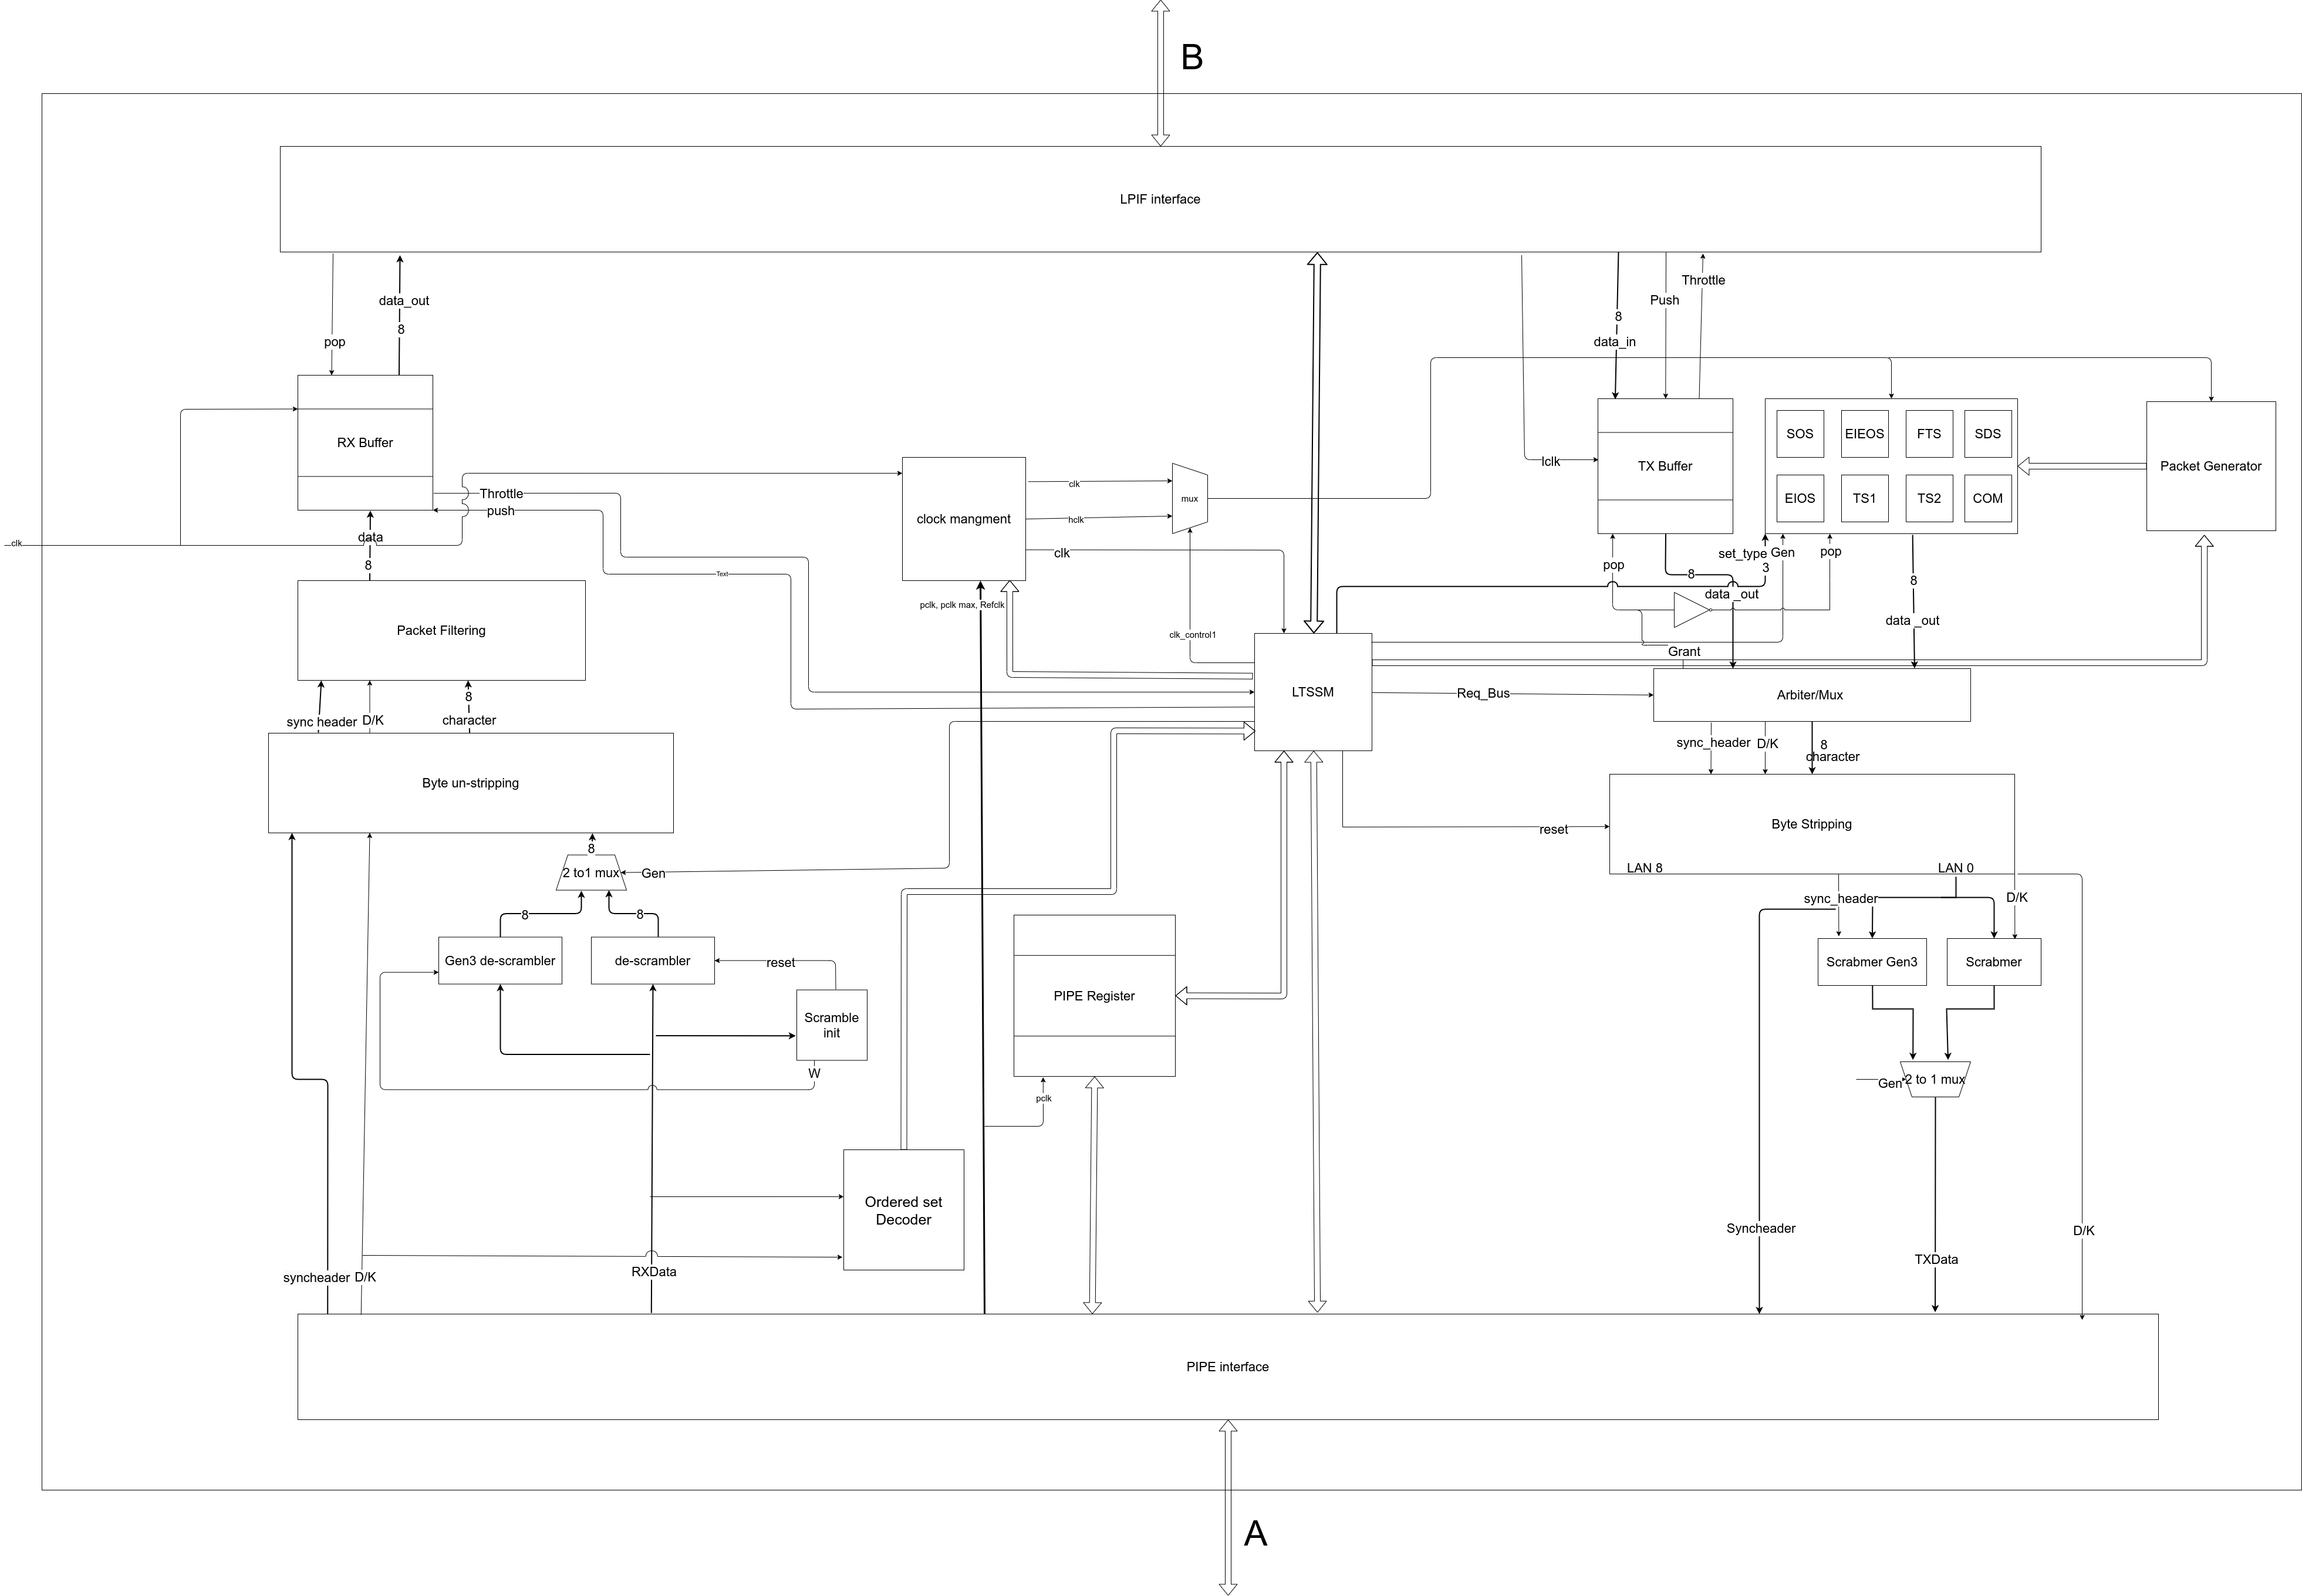
\includegraphics[width=130mm,height=130mm]{images/design-abstract (2).png}
  \caption{MAC Layer Architecture}
  
  \label{fig:arch}
\end{figure}

\subsection{LTSSM}
 \begin{itemize}
     \item Contain Active State Power Management which responsible for power states of the device.
     \item change link width and bit rate. 
     \item send parameters( lane and link number, ....) to Generate Packet module to generate required ordered sets. 
     \item send Req\_Bus signal to arbiter/mux to choose between ordered sets or packet symbol.
     \item choose PCIe generation mode.
 \end{itemize}
 
 \subsection{PIPE Interface}
 It Contains 4 main modules each:
 \begin{itemize}
     \item Rx module \newline
     It receives data from PCS layer in signal RXData and contains Rx related signals(RXsybcheader, RXDatak, .....) see Table \ref{tab:p2}
     \item Tx module \newline
     It tramsites data to PCS layer in signal TXData and contains Tx related signals(TXsybcheader, TXDatak, .....) see Table \ref{tab:p1}
     \item Error handler \newline
     It receives all error signals and generate responde to LTSSM 
    % \item Control unit \newline
    % Encode and Decode message bus \textbf{}
     Note: signal details in Section \ref{sec:1}
     
  \begin{figure}[H]
  \centering
  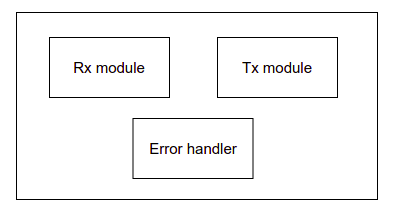
\includegraphics{images/pipe_interface.png}
  \caption{PIPE interface}
  
  \label{fig:pipe}

  
\end{figure}


 \end{itemize}
 
  \subsection{LPIF Interface}
  
  \begin{itemize}
      \item   LPIF Error handler receives all error signals then make some process to send decision to  LPIF ctl 
        \item LPIF ctl control  Txbuffer and Rxbuffer based on error and status signals and send his status to LTSSM to control other modules based on this situation 
  \end{itemize}

  \begin{figure}[H]
  \centering
  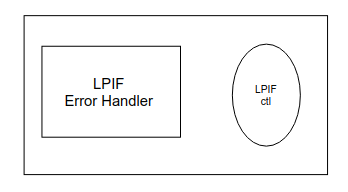
\includegraphics{images/lpif_1.png}
  \caption{LPIF interface}
  
  \label{fig:pipe}
\end{figure}

\subsection{Scrambler init}
\begin{itemize}
    \item COM Detector \newline
    Detect 6 COM symbols to reset scrambler in gen 1,2
    \item SKP Detector \newline
    Detect skp ordered set based on this it sets $W$ signal which next value LFSR is taked as a seed to scrambler gen 3
\begin{figure}[H]
  \centering
  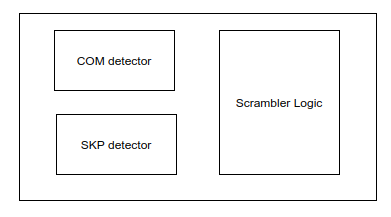
\includegraphics[height=50mm,width=100mm]{images/init.png}
  \caption{Scrambler init}
\end{figure}

\end{itemize}


\subsection{Ordered set and packet Generator module}
\begin{itemize}
    \item Ordered Set module \newline It contains 6 orederd sets end each set has two generation packets. 
\item Packet Generator module \newline It is responsible to  generate gen 3 ordered sets.
\end{itemize}

\begin{figure}[H]
  \centering
  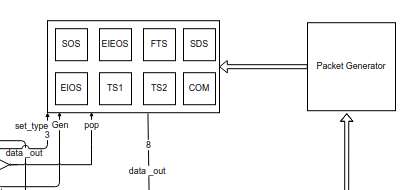
\includegraphics{images/ordered_set.png}
  \caption{Ordered set and packet Generator module}
\end{figure}


\begin{table}[H]
    \caption{Input signals for ordered set module}
    \centering
  \begin{tabular}{ |m{26mm}|m{60mm}|  }
\hline
\rowcolor{Gray}
\multicolumn{1}{|c|}{\textbf{Name} } 
& \multicolumn{1}{|c|}{\textbf{Description}}\\
\hline
 set\_type  &  choose ordered set type (SOS, EIEOS, ....) \\ \hline 
  Gen & choose generation of the packet gen 1$\longrightarrow $2 or gen 3$\longrightarrow$5 \\ 
 \hline 
 pop & It pops the packet to the bus (data\_out) symbol by symbol until finish \\
 \hline 


\end{tabular}
\end{table}


\chapter{Scenarios}
\section{PIPE interface scenarios}

    \subsection{Electrical Idle} 
    The base spec requires that devices send an Electrical Idle ordered set before Tx+/Tx- goes to the electrical idle state.
    \begin{itemize}
        \item The general rules for entring electrical idle state :
\begin{itemize}
    \item Strat sending EIOS with asserting TxDataK at the same time.
\item the MAC must always align the electrical idle ordered set on the parallel interface so the first byte of the ordered set is always on the low-order data lines (TxDataK[7:0]).

\item Assert TxElecIdle just after sending the EIOS and make sure that TxDataValid is asserted whenever TxElecIdle toggles.

\end{itemize}
\item 
The following timing diagram shows an example of electrical idle entry for gen1,2:

\begin{figure}[H]
  \centering
  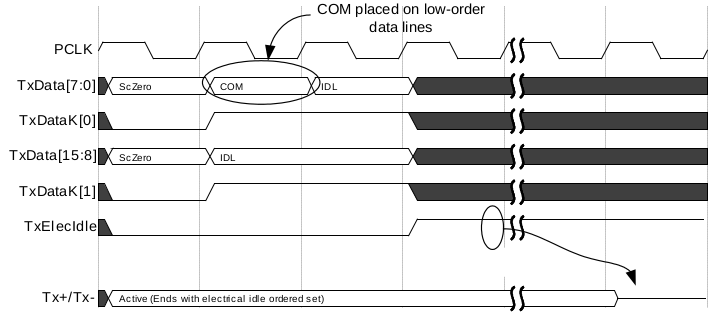
\includegraphics[width=130mm,height=60mm]{images/clk_diagram/EI.png}
  \caption{electrical idle entry for gen1,2}
\end{figure}
\item Some notes on the previous example :
\begin{itemize}
    \item COM appears on the low-order data lines (TxDataK[7:0]).
\item TxElecIdle is asserted after finishing the EIOS.
\item TX+/TX- leaves Active state with the end of EIOS.

\end{itemize}
\item The general rules for leaving electrical idle state :
\begin{itemize}
    \item De-assert TxElecIdle and start sending data.
    \item Make sure TxDataValid is asserted to ensure sampling TxElecIdle.

\end{itemize}
\item The following timing diagram shows an example of electrical idle entry for gen 3:
\begin{figure}[H]
  \centering
  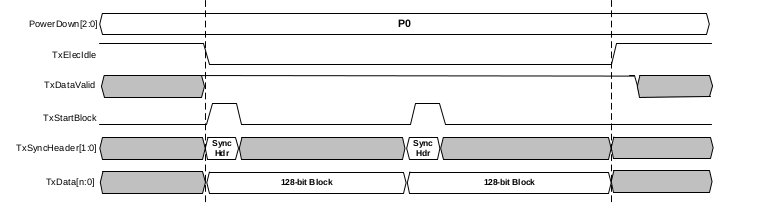
\includegraphics[width=130mm,height=60mm]{images/clk_diagram/EIGen3.png}
  \caption{electrical idle entry for gen3}
  \label{lane}
\end{figure}
Some notes on the previous example:
\begin{itemize}
    \item TxDataValid can assert earlier before TxElecIdle toggles.

    \item TxDataValid can de-assert anytime after TxElecIdle asserts as long as it does not overlap with the next Electrical Idle exit sequence.

    \item TxElecIdle must de-assert at the same clock TxStartBlock asserts.



\end{itemize}
    \end{itemize}
\subsection{Link Equalization Evaluation} 
\begin{itemize}
    \item While in the P0 power state, the PHY can be instructed to perform evaluation of the current TX equalization settings of the link partner.
    \item Basic operation of the equalization evaluation is that:
\begin{itemize}
    \item the MAC requests the PHY to evaluate the current equalization settings by asserting RxEqEval.
    \item When the PHY has completed evaluating the current equalization settings, it asserts PhyStatus for one clock

    \item The PHY drives the LinkEvaluationFeedback signals to the appropriate feedback response.

    \item The MAC must deassert RxEqEval before initiating another evaluation.

    \item To abort an evaluation the MAC de-asserts RxEqEval before the PHY has signaled completion. If the MAC aborts the evaluation the PHY must signal completion as quickly as possible. The MAC ignores returned evaluation values in an abort scenario.
\item If a race condition occurs where the MAC aborts by deasserting RxEqEval on same cycle as the PHY asserts PhyStatus then the PHY shall not take any further action.


\end{itemize}
\item The next figure shows an example of the timings for a successful link equalization evaluation request:
\begin{figure}[H]
  \centering
  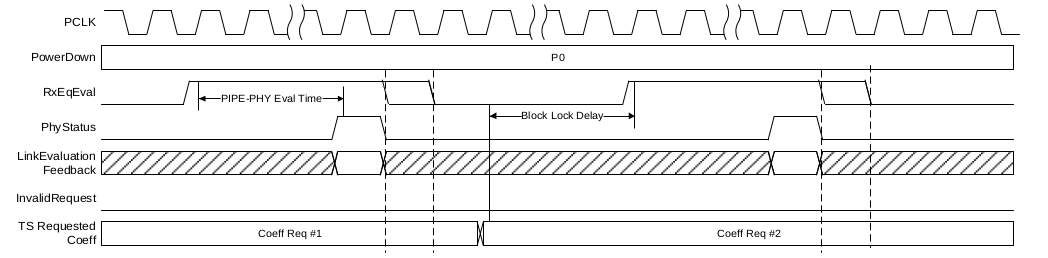
\includegraphics[width=130mm,height=60mm]{images/clk_diagram/eq.png}
  \caption{successful link equalization evaluation request}
  \label{lane}
\end{figure}
\item Notes :
\begin{itemize}
    \item RxEqEval can de-assert at the same clock the corresponding PhyStatus de-asserts or later as long as RxEqEval de-asserts prior to the next RX Equalization Request.

    \item Back-to-back RxEqEval request can happen as close as one clock apart (i.e. RxEqEval can de-assert for one clock before it re-asserts again to start the next RX Equalization request.

    \item Once the MAC has requested link equalization evaluation (by asserting RxEqEval), the MAC must leave RxEqEval asserted until after the PHY has signaled completion by the assertion of PhyStatus unless the MAC needs to abort the evaluation due to high level timeouts or error conditions.

\end{itemize}

    \item The next figure shows PCI Express 3.0 Equalization Evaluation Request Resulting in Invalid Feedback
\begin{figure}[H]
  \centering
  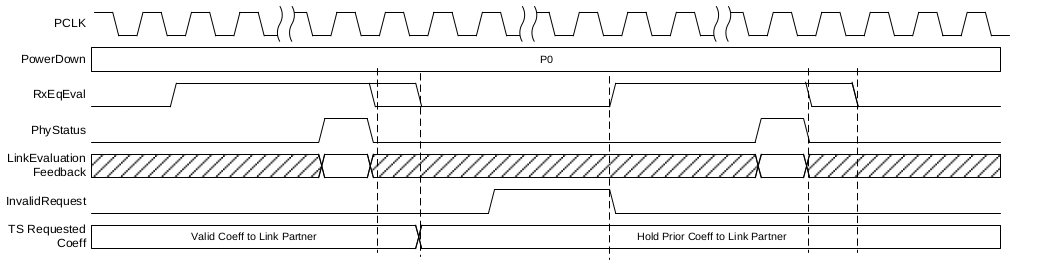
\includegraphics[width=130mm,height=60mm]{images/clk_diagram/eq_v.png}
  \caption{Equalization Evaluation RequestResulting in Invalid Feedback}
  \label{lane}
\end{figure}

\end{itemize}
\subsection{Active PM L0 to L0s and back to L0}  
\begin{itemize}
    \item When the MAC and higher levels have determined that the link should transition to L0s, the MAC transmits an electrical idle ordered set and then has the PHY transmitter go idle and enter P0s.
\item The general rules for entering L0s state from L0:
\begin{itemize}
    \item MAC sends EIOS with the same rules mentioned in the  Electrical Idle section.
\item Just after sending the EIOS, the MAC changes PowerDown[1:0] to 01b indicating transitioning to L0s.
\end{itemize}
The next figure shows the L0s entry for PCIe gen1/2:
\begin{figure}[H]
  \centering
  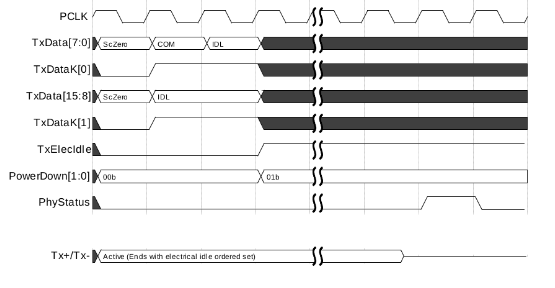
\includegraphics[width=130mm,height=60mm]{images/clk_diagram/l0.png}
  \caption{L0s entry for PCIe gen1/2}
  \label{lane}
\end{figure}
\item The general rules for exiting L0s state to L0:
\begin{itemize}
    \item The MAC transitions the PHY from the P0s state to the P0 state by changing PowerDown[1:0] to 00b.
\item The MAC waits for the PHY to indicate that it is ready to transmit (by the assertion of PhyStatus).
\item Then the MAC begins transmitting Fast Training Sequences (FTS).

\item The next figure shows an example of L0s to L0 transition when the PHY is running at 2.5GT/s.

\begin{figure}[H]
  \centering
  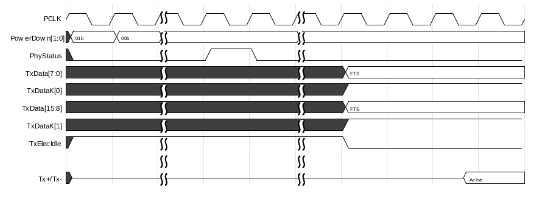
\includegraphics[width=130mm,height=60mm]{images/clk_diagram/l0g.png}
  \caption{ L0s to L0 transition}
  \label{lane}
\end{figure}

\end{itemize}
\end{itemize}
\subsection{reestablish block alignment in recovery state} 
\begin{itemize}
    \item L0 state --> Recovery state due to loss of alignment is detected

    \item In Recovery.RcrLck/cfg, Mac layer assert commandBlockAlignControl bit using messagebus:
\begin{itemize}
    \item Send write committed message to change PHY RX Control4 register to h01 on M2P\_Messagebus.
    \item The phy send ack back for this message on P2M\_Messagebus

    
\end{itemize}
    \item PHY while (commandBlockAlignControl asserted) search for EIEOS to achieve
   block alignment

    \item After Blockalignment is finished

    \item Mac layer go to status L0 and deassert commandBlockAlignControl bit using messagebus:
\begin{itemize}
    \item Send write committed message to change PHY RX Control4 register to h00 on M2P\_Messagebus
\item The phy send ack back for this message on P2M\_Messagebus

\begin{figure}[H]
  \centering
  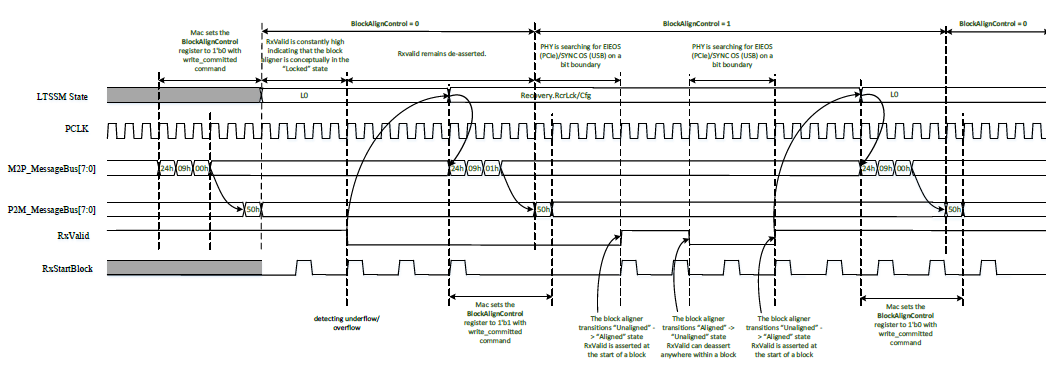
\includegraphics[width=130mm,height=60mm]{images/clk_diagram/recovery.png}
  \caption{reestablish block alignment in recovery state}
  \label{lane}
\end{figure}
\end{itemize}
\end{itemize}
\subsection{RXeqTraining} 
\begin{itemize}
    \item IN Recovery.Equalization Substate,Mac start EqTraining by asserting RXEqTraining bit using messagebus:
\begin{itemize}
    \item Send write committed message to change PHY RX Control1 register[0] to 1 on M2P\_Messagebus
\item The phy send ack back for this message on P2M\_Messagebus 

\end{itemize}
    \item When PHY complete Equalization Training 
    \item PHY layer indicate the status of completion to MAC layer via RxEqualizationDone bit using messagebus:
    \begin{itemize}
        \item  Send write committed message to change RX status register to 1  on P2M\_Messagebus
    \item The Mac send ack back for this message on M2P\_Messagebus


    \end{itemize}
    \begin{figure}[H]
  \centering
  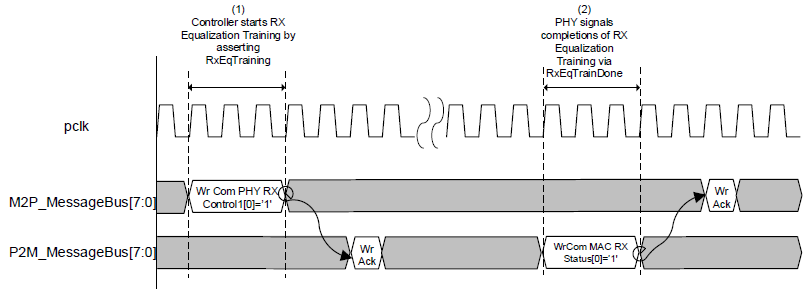
\includegraphics[width=130mm,height=60mm]{images/clk_diagram/RXeqTraining.png}
  \caption{RXeqTraining}
  \label{lane}
\end{figure}
    
\end{itemize}
 \subsection{Reset}
\begin{itemize}
    \item The MAC reset the PHY by asserting Reset signal (active low). 
    \item While Reset is asserted the MAC should have TxDetectRx/Loopback deasserted, TxElecIdle asserted, TxCompliance deasserted and the PowerDown = P1.
    \item For initial power on the MAC must holds PHY in reset until the power and CLK to the PHY are stable.
    \item The PhyStatus is signal is high during reset until reset is deasserted and PCLK is running in operational frequency for one cock and the PHY is in specified power state then it will be deasserted.
    \item When PhyStatus deasserted after the deassertion of the Reset, The MAC can perform any operational sequences.

\begin{figure}[H]
  \centering
  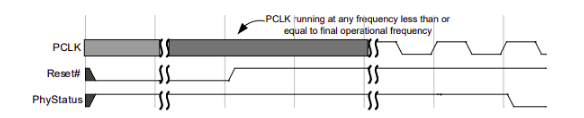
\includegraphics[width=160mm,height=40mm]{images/clk_diagram/reset.png}
  \caption{Reset}
  \label{lane}
\end{figure}
\end{itemize}
\subsection{Updating TxDeemph}  
The TXDeemph is 18-bit variable divided into three parts on (PHY TX Control2, PHY TX Control3, PHY TX Control4) registers.
\begin{itemize}
    \item The MAC sends on M2P\_MessageBus write\_committed to TxControl5 register to make GetLocalPresetCoefficients request for one or more values of LocalPresetIndex to update the TxDeemph value.
This field is used to make dynamic preset coefficient updates.
\item The PHY acknowledge the request by sending write\_ack on the P2M\_MessageBus.
\item The PHY sends three messages on the P2M\_MessageBus to update the LocalPresetCoefficients fields in the (Tx Status0, Tx Status1, Tx Status2) registers.
\item The MAC sends write\_ack message on M2P\_MessageBus to ensure that the LocalPresetCoefficients fields are updated successfully.
\item The MAC sends three messages on the M2P\_MessageBus to the PHY.
\begin{itemize}
    \item Two of them are write\_ucommitted.

    \item One write\_committed to ensure that data are written in the (PHY TX Control2, PHY TX Control3, PHY TX Control4) registers. 

    \item for TxDeemph, the new TxDeemph value must be reflected on the pins within 128ns.
\end{itemize}
\item After the write\_committed for TxDeemph, the new TxDeemph value must be reflected on the pins within 128ns. \newline \newline 

Note: For every GetLocalPresetCoefficients request, there is a 128ns maximum response time for the PHY to return the LocalTxPresetCoefficients value. 

\begin{figure}[H]
  \centering
  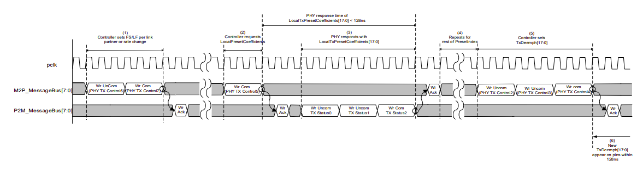
\includegraphics[width=150mm,height=50mm]{images/clk_diagram/deemph.png}
  \caption{Updating TxDeemph}
  \label{lane}
\end{figure}


\end{itemize}
\subsection{Selecting De-emphasis} 
\begin{itemize}
    \item While in the P0 power state and transmitting at 5.0GT/s, 8.0 GT/s, 16 GT/s or 32 GT/s, the PHY can be instructed to change the value of the transmitter equalization.
\item Steps of operation:
\begin{itemize}
    \item The MAC changes the TXDeemph value with the new Tx-De-emphasis value.

    \item If the signaling rate is 5GT/S, the PHY must be capable of transmitting with the new setting within 128 ns.
    \item If the signaling rate is 8.0 GT/s, 16 GT/s, or 32 GT/s, the PHY must be capable of transmitting with the new setting within 256 ns.

\end{itemize}
\begin{figure}[H]
  \centering
  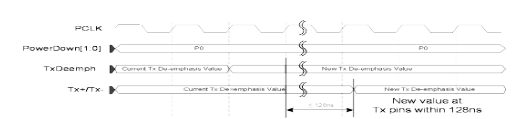
\includegraphics[width=130mm,height=50mm]{images/clk_diagram/de.png}
  \caption{Selecting Tx De-emphasis value}
  \label{lane}
\end{figure}
\end{itemize}
\item Polarity Inversion
\begin{itemize}
    \item RxPolarity signal must be asserted to make polarity inversion.

    \item The PHY must invert received data after RxPolarity is asserted.

    \item Inverted data must be showing up on RxData within 20 PCLKs after the assertion of RxPolarity.

    \item Note: The D21.5 symbol when inverted it will be D10.2 symbol as shown in figure.
\begin{figure}[H]
  \centering
  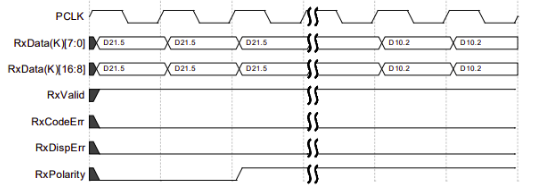
\includegraphics[width=140mm,height=50mm]{images/clk_diagram/p.png}
  \caption{Polarity inversion}
  \label{lane}
\end{figure}
\end{itemize}
\subsection{Signal rate}
\begin{itemize}
    \item Signal rate can be change when PHY in L0 or L1 power state and Tx Electrical IDL is asserted.

    \item After the MAC changes PCLK rate, the change to the PCLK can happen only after the PclkChangeOk has been driven high by the PHY.

    \item The MAC changes the input PCLK and then handshakes by asserting PclkChangeAck.

    \item The PHY responds by the asserting PhyStatus for one input PCLK cycle and deasserts PclkChangeOk on the trailing edge of PhyStatus.

    \item The MAC deasserts PclkChangeAck when PclkChangeOk is sampled low and may deassert Tx Electrical IDL.

\begin{figure}[H]
  \centering
  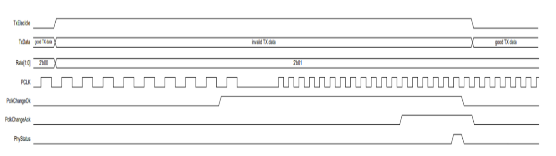
\includegraphics[width=130mm,height=50mm]{images/clk_diagram/rate.png}
  \caption{signal rate}
  \label{lane}
\end{figure}
\end{itemize}
\subsection{Error Detection} 
\begin{itemize}
    \item The PHY is responsible for detecting receive errors of several types, these errors are signalled to the MAC layer using the receiver status signals (RxStatus[2:0]).

    \item When a receive error occurs, the appropriate error code is asserted for one clock cycle at the point in the data stream across the parallel interface closest to where the error actually occurred.

    \item There are four error conditions that can be encoded on the RxStatus signals.

    \item If more than one error should happen to occur on a receive byte, the errors should be signaled with the priority shown below.
\begin{itemize}
    \item 8B/10B decode error or block code error (RxStatus=100b).

    \item Elastic Buffer overflow (RxStatus=101b).

    \item Elastic Buffer underflow (RxStatus=110b).

    \item Disparity errors (RxStatus=111b).

\end{itemize}
\end{itemize}
\subsection{8B/10B Decode Errors} 
\begin{itemize}
    \item For a detected 8B/10B decode error, the PHY should place an EDB symbol in the data stream in place of the bad byte, and encode RxStatus with a decode error during the clock cycle when the effected byte is transferred across the parallel interface. 

    \item For greater than 8-bit interface, if the bad on the lower byte lane, one of the other bytes may have bad disparity, but the 8B/10B error has the precedence.

    \item In the example below, the receiver is receiving a stream of bytes Rx-a through Rx-z, and byte Rx-f has an 8B/10B decode error, in the place of that byte, the PHY places an EDB on the parallel interface and sets RxStatus to the 8B/10B decode error code.
\begin{figure}[H]
  \centering
  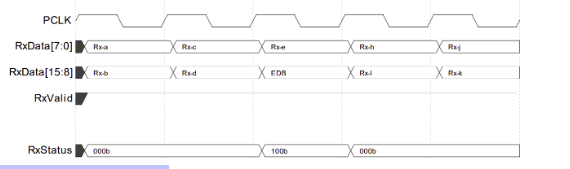
\includegraphics[width=130mm,height=50mm]{images/clk_diagram/dr.png}
  \caption{8B/10B Decode Errors}
  \label{lane}
\end{figure}
\end{itemize}
\subsection{Disparity Errors} 
\begin{itemize}
    \item For a detected disparity error the PHY should assert RxStatus with the disparity error code during the clock cycle when the affected byte is transferred across the parallel interface.
 
    \item For greater than 8-bit interfaces, it is not possible to discern which byte (or possibly both) had the disparity error.

    \item In the example below, the receiver detected a disparity error on either (or both) Rx-e or Rx-f data bytes and indicates this with the assertion of RxStatus.

\begin{figure}[H]
  \centering
  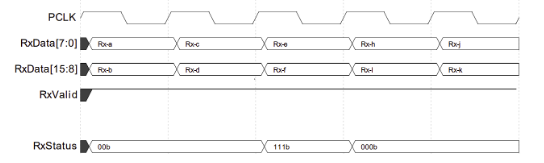
\includegraphics[width=130mm,height=50mm]{images/clk_diagram/disparity.png}
  \caption{Disparity Errors}
  \label{lane}
\end{figure}
\item  Note: MACs often treat 8B/10B errors and disparity errors identically.
\end{itemize}


\subsection{Elastic Buffer Errors}
\subsubsection{Elastic Buffer Underflow}

\begin{itemize}
    \item For elastic buffer errors, an underflow should be signaled during the clock cycle or clock cycles when a spurious symbol is moved across the parallel interface, the symbol moved across the interface should be the EDB symbol.

    \item In the timing diagram below, the PHY is receiving a repeating set of symbols Rx-a thru Rx-z, the elastic buffer underflows causing the EDB symbol to be inserted between Rx-g and Rx-h symbols, the PHY drives RxStatus to indicate buffer underflow during the clock cycle when the EDB is presented on the parallel interface.

\end{itemize}




\begin{figure}[H]
  \centering
  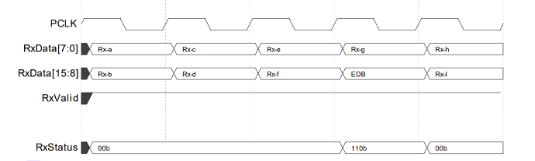
\includegraphics[width=130mm,height=50mm]{images/clk_diagram/underflow.png}
  \caption{Elastic Buffer Underflow}
  \label{lane}
\end{figure}
\subsubsection{Elastic Buffer Overflow}
\begin{itemize}
    \item For an elastic buffer overflow, the overflow should be signaled during the clock cycle where the dropped symbol or symbols would have appered in the data stream.

    \item For the 16-bit interface it is not possible, or necessary, for the MAC to determine exactly where in the data stream the symbol was dropped.

    \item In the timing diagram below, the PHY is receiving a repeating set of symbols Rx-a thru Rx-z, the elastic buffer overflows causing the symbol Rx-g to be discarded, The PHY drives RxStatus to indicate buffer overflow during clock cycle when Rx-g would have appeared on the parallel interface.     

\end{itemize}




\begin{figure}[H]
  \centering
  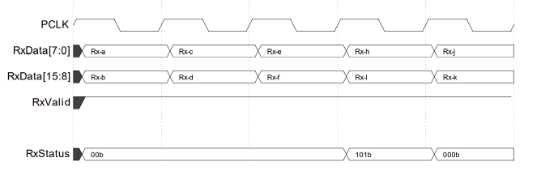
\includegraphics[width=130mm,height=50mm]{images/clk_diagram/overflow.png}
  \caption{Elastic Buffer Overflow}
  \label{lane}
\end{figure}
\subsection{Receiver detection}
\begin{itemize}
    \item While in the P1 power state the PHY can be instructed to perform a  receiver detection operation to determine if there is a receiver at the other end of the link.

    \item Basic operation of receiver detection is that MAC requests the PHY to do receiver detect sequence by asserting TxDetectRx/Loopback.

    \item When the PHY has completed the receiver detect sequence, it asserts PhyStatus for one clock and drives the RxStatus signals to the appropriate code.

    \item After the receiver detection has completed, the MAC must deassert TxDetectRx/Loopback before initiating another receiver detection.

    \item Once the MAC has requested a receiver detect sequence the MAC must leave TxDetectRx/Loopback asserted until after the PHY has signaled completion by the assertion of Phystatus.
\end{itemize}




\begin{figure}[H]
  \centering
  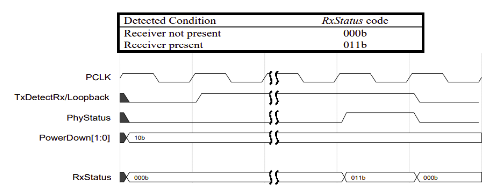
\includegraphics[width=130mm,height=50mm]{images/clk_diagram/detection.png}
  \caption{Receiver detection}
  \label{lane}
\end{figure}

\subsection{128b/130b Encoding and Block synchronization}
\begin{itemize}
    \item For every block (usually 128 bits) that is moved across the PIPE TxData interface at the 8.0 GT/s rate, 16 GT/s rate, or 32 GT/s rate, TxSyncHeader signal is asserted to Provide the Sync Header for the PHY to use in the next 128b block.

    \item The MAC must assert the TxDataValid signal to indicate that PHY will use the data.
    \item TxStartBlock signal is asserted to allow the MAC to tell PHY the starting byte for a 128b block.

    \item TxElecIdle signal Forces Tx output to electrical idle when asserted.

    \item For every block (usually 128 bits) that is moved across the PIPE RxData interface at the 8.0 GT/s rate, 16 GT/s rate, or 32 GT/s rate, RxSyncHeader signal is asserted to Provide the Sync Header for the MAC to use in the next 128b block.

    \item The PHY must assert the RxDataValid signal to indicate that MAC will use the data.

    \item RxStartBlock signal is asserted to Allows the PHY to tell MAC the starting byte for a 128b block.

    \item RxElecIdle signal Indicates receiver detection of an electrical idle when asserted.
\end{itemize}
\begin{figure}[H]
  \centering
  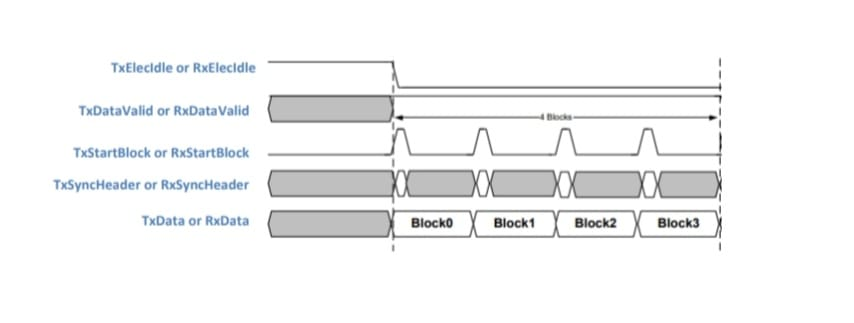
\includegraphics[width=130mm,height=50mm]{images/clk_diagram/end.jpeg}
  \caption{128b/130b Encoding and Block synchronization}
  \label{lane}
\end{figure}

% \begin{figure}[H]
%   \centering
%   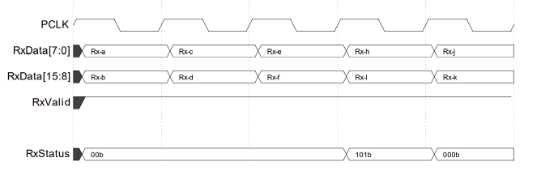
\includegraphics[width=130mm,height=50mm]{images/clk_diagram/overflow.png}
%   \caption{Elastic Buffer Overflow}
%   \label{lane}
% \end{figure}
\end{document}
